% ---- ETD Document Class and Useful Packages ---- %
\documentclass{ucetd}
\usepackage{subfigure,epsfig,amsfonts}
\usepackage{natbib}
\usepackage{amsmath}
\usepackage{amssymb}
\usepackage{amsthm}

\usepackage{url}


%% Use these commands to set biographic information for the title page:
\title{Stochastic computation in recurrent networks of spiking neurons}
\author{Clayton W. Seitz}
\department{Graduate Program in Biophysics}
\division{Physical and Biological Sciences}
\degree{Master of Science}
\date{Winter 2021}

%% Use these commands to set a dedication and epigraph text

\epigraph{Epigraph}

\begin{document}
%% Basic setup commands
% If you don't want a title page comment out the next line and uncomment the line after it:
\maketitle
%\omittitle

% These lines can be commented out to disable the copyright/dedication/epigraph pages
\makecopyright
%\makededication
\makeepigraph


%% Make the various tables of contents
\tableofcontents
%\listoffigures
%\listoftables

\acknowledgments
% Enter Acknowledgements here

\abstract

The primate cerebral cortex is a complex system estimated to harbor more than 25 billion neurons communicating via action potentials or `spikes' and is responsible for many higher-order brain functions including memory and learning. Recent years have hosted many efforts to understand how such complex phenomena emerge from the communication of individual cells. Many studies have provided evidence that long term plasticity (LTP) in synapses permits a long-lasting alteration of network dynamics and, in turn, forms the basis of long-term memory and learning. However, understanding memory formation and learning in the brain is made difficult by the variability in the response of cortical neurons to stimuli. Therefore, capturing the apparent stochastic features of neural activity in computer based models, such as recurrent spiking neural networks (RSNNs), while explaining their manipulation of information mathematically has become the gold standard for computational neuroscience. Models of neural networks derived from statistical mechanics, such as those which assert that the membrane potential of a cortical neuron obeys a form of Langevin dynamics, can potentially account for stochastic network activity. Such models also provide the intriguing interpretation that neural activity represents sampling from a probability distribution - a technique central to statistical inference.  Here, we apply a similiar mathematical treatment to the study of an RSNN by modeling the membrane potential statistics of an integrate and fire neuron using Fokker-Planck equations. With this statistical framework in hand, we can recast a network of neurons as a stochastic process in higher dimensions and explore the relationships between synaptic connectivity and its plasticity to the correlation structure of neural spike trains. This approach is also amenable to information theoretic analysis and is a step toward a mathematical relationship between neuroplasticity mechanisms and the emergent computational capabilities of cortical microcircuits.



\mainmatter

\chapter{Introduction}

Towards the Hopfield network [2] which spawned an entire field of research applying techniques from the statistical physics of spin glasses to the description of neural activity. A popular approach towards the end of 20th century simplified a network of neurons firing action potentials to an ensemble of coupled spins obeying an energy function over the space of states. , the Hopfield model related the patterns learned by a network to the energy landscape over the discrete space of states. The storage capacity of these networks and the geometry of this energy landscape were of particular interest and rigorous mathematical treatment has been used to show limits on the basins of attraction in such energy landscapes [4,10,11]. However, recent experimental evidence has suggested that networks of neurons may follow a stochastic, rather than deterministic, computational paradigm. There are many examples in the literature of trial-to-trial variability in the response of cortical neurons to identical stimuli, suggesting that computations in the brain are inherently stochastic. The origins of this stochasticity are hypothesized to originate in noise in synaptic conductances and infidelity in processes clearing neurotransmitters from the synaptic cleft. Interestingly, an extension of the Hopfield model - the Boltzmann machine actually leverages stochastic activity of Ising spins to perform powerful computations [14]. In such a model, the set of synaptic weights $\Phi$ ``embody" the joint distribution $P_{\Phi}(X,R) = P_{\Phi}(X)P_{\Phi}(R|X)$ over network inputs and network response, respectively. Then, computations can be viewed as probabilistic inference after suitable transformations of the weights $\Delta\Phi$. Such physically inspired models have proven useful; however, the models are sufficiently abstract to make experimental comparisons difficult. More recent endeavors appear to make useful predictions on network dynamics by using Fokker-Planck equations to compute distributions of the membrane voltage as a function of time [5]. Here, we apply a similar formalism to the description of network dynamics with heterogeneous and stochastic synaptic weights to probe the distribution over network states $P_{\Phi}(R)$ and describe how this framework can be used to provide insights on how the neural networks embody the distribution $P_{\Phi}(R|X)$ in statistical inference tasks. To conclude, we discuss the effect of synaptic plasticity.


The quantitative discussion of the dynamics of many complex systems (systems where the number of interacting units $N$ is large) in nature from networks of spiking neurons, geophysical systems, to excitable media, all necessarily require a statistical description. Indeed, enumerating the available states to such a system itself has proven intractable, even for small systems over short time scales. As an example, consider the states of an interacting system of $N$ binary variables denoted $\{z_{i}\}_{i=1}^{N}$ which might be physically realized as an ensemble of spins in a ferromagnet. Even for extremely small cases such as $N=100$ the system can take on $2^{100} = 1.26\times 10^{30}$ different configurations and by $N=300$ the number of configurations exceed our best estimates for the number of atoms in the known universe. At the same time, we cannot hope to make enough measurements of such a system to estimate the probability distribution over the space of states and make inferences on the organization and interactions of the individual elements based on such a distribution. We can, however, develop model distributions over the available states based on stochastic interaction between the individual units that account for the degrees of freedom which we cannot approach analytically - a technique often employed in the description of the statistical physics of particles. This family of techniques, often formally referred to as Langevin dynamics, is defined by the use of stochastic differential equations to model the evolution of systems with high degrees of freedom. A Fokker-Planck equation allows us to solve for the time evolution of the probability distribution over such a variable, providing insights into the dynamics which cannot be seen from any one trajectory through the space of states. 

\chapter{Stochastic systems and Fokker-Planck equations}

\section{The Langevin Equation}



In the context of neuroscience, the Fokker-Planck approach has been taken by many in describing the dynamics of the membrane potential distribution in a population of neurons. In the following paragraphs, we will sketch a derivation of the Fokker-Planck equation for a general stochastic process in one dimension and apply this result to networks of integrate and fire neurons.

\subsection{The Kramers-Moyal expansion}

Given many instantiations of a stochastic variable $V$, we can construct a normalize histogram over all observations as a function of time $P(V,t)$. However, in order to systematically explore the relationship between the parameterization of the process and $P(V,t)$ we require an expression for $\dot{P}(V,t)$. If we make a fundamental assumption that the evolution of $P(V,t)$ follows a Markov process i.e. its evolution has the memoryless property, then we can write

\begin{equation}
P(V', t) = \int T(V', t | V, t-\tau)P(V, t-\tau)dV
\end{equation} 

which is known at the Chapman-Kolmogorov equation. The factor $T(V', t | V, t-\tau)$ is known as the \emph{transition operator} in a Markov process and determines the evolution of $P(V,t)$ in time. We proceed by writing $T(V', t | V, t-\tau)$ in a form referred to as the Kramers-Moyal expansion

\begin{align*}
T(V', t | V, t-\tau) &= \int \delta(u-V')T(u, t | V, t-\tau)du\\
&= \int \delta(V+u-V'-V)T(u, t | V, t-\tau)du\\
\end{align*} 

If we use the Taylor expansion of the $\delta$-function 

\begin{equation*}
\delta(V+u-V'-V) = \sum_{n=0}^{\infty} \frac{(u-V)^{n}}{n!}\left(-\frac{\partial}{\partial V}\right)^{n}\delta(V-V')
\end{equation*}

Inserting this into the result from above, pulling out terms independent of $u$ and swapping the order of the sum and integration gives

\begin{align}
T(V', t | V, t-\tau) &= \sum_{n=0}^{\infty} \frac{1}{n!}\left(-\frac{\partial}{\partial V}\right)^{n}\delta(V-V')\int(u-V)^{n}T(u, t | V, t-\tau)du\\
&= \sum_{n=0}^{\infty} \frac{1}{n!}\left(-\frac{\partial}{\partial V}\right)^{n}\delta(V-V')M_{n}(V,t)
\end{align} 

noticing that $M_{n}(V,t) = \int(u-V)^{n}T(u, t | V, t-\tau)du$ is just the $n$th moment of the transition operator $T$. Plugging (2.6) back in to (2.4) gives 

\begin{align}
P(V, t) &= \int \left(1 + \sum_{n=1}^{\infty} \frac{1}{n!}\left(-\frac{\partial}{\partial V}\right)^{n} M_{n}(V,t)\right)\delta(V-V')P(V, t-\tau)dV\\
&= P(V', t-\tau) + \sum_{n=1}^{\infty} \frac{1}{n!}\left(-\frac{\partial}{\partial V}\right)^{n} \left[M_{n}(V,t)P(V,t)\right]
\end{align} 

Approximating the derivative as a finite difference and taking the limit $\tau\rightarrow 0$ gives

\begin{align}
\dot{P}(V,t)  &= \underset{\tau\rightarrow 0}{\mathrm{lim}}\left(\frac{P(V, t)-P(V, t-\tau)}{\tau}\right)\\
&= \sum_{n=1}^{\infty} \frac{1}{n!}\left(-\frac{\partial}{\partial V}\right)^{n} \left[M_{n}(V,t)P(V,t)\right]
\end{align} 

which is formally known as the Kramers-Moyal (KM) expansion. The Fokker-Planck equation is a special case of (2.10) where we neglect terms $n>2$ in the \emph{diffusion approximation}.

\subsection{A network of leaky integrate and fire neurons}

We consider a general network of $N$ leaky integrate and fire units expressed mathematically as a weighted graph $\mathcal{N}$. We defined the state vector $\mathbf{V}$ that stores the membrane potential of each cell, which evolves according to a set of $N$ coupled differential equations

\begin{align*}
\dot{V_{j}}(t) = -\frac{V_{j}(t)}{\tau} + \sum_{i}J_{ij}\delta(t-t_{spike}) + X_{j}(t)
\end{align*}

for a stochastic input $X$, which we assume can be written as a compound Poisson process, and a weighted summation of spikes in the primary population $\sum_{i}J_{ij}\delta(t-t_{spike})$. The state vector for the system is then $\mathbf{V}(t) = (V_{0}(t), V_{1}(t), ..., V_{N}(t))$ and we look for an analytical relationship between the joint distribution $P(\mathbf{V}(t))$ and the synaptic connectivity $J$. In principle, if we know the moments $\{M_{j}^{n}\}$  of the transition operator $T_{j}(V',t'|V,t)$ for every neuron $j$ to arbitrary order, we can express $\dot{P}(\mathbf{V}(t))$ according to the KM expansion in (2.7). The primary hurdle we need to overcome in this procedure then becomes relating the moments $\{M_{j}^{n}\}$ to the synaptic connectivity $J$. For example, we can construct a general template for the distribution $T_{j}$ by noticing that the probability of a binary input pattern

\begin{align*}
P(\mathbf{z}) = \underset{j}{\prod} \; p_{j}^{z_{j}}(1-p_{j})^{1-z_{j}}
\end{align*}

which is a multivariate Bernoulli distribution. If we let $\xi$ index the space of possible binary patterns

\begin{align}
T(V',t'|V,t) = \sum_{\xi} \delta(V'- V - J\cdot z_{\xi})\underset{j}{\prod} \; p_{j}^{z_{j}}(1-p_{j})^{1-z_{j}}
\end{align}

so we see that we must first know $P(\mathbf{z})$ which in turn requires knowledge of all $p_{j} = P_{j}(\theta, t)$ i.e. the probability flux at the threshold $\theta$. We now argue that the moments of (2.8) can be found 

\begin{align}
M_{n} = \int (V-V')^{n} T(V',t'|V,t) dV
\end{align}

which are essentially the moments of a compound Bernoulli distribution where the individual probabilities $p_{j}(t')$ are given by $P_{j}(\theta, t)$.



\subsection{The Ornstein-Uhlenbeck Prototype}

The Ornstein-Uhlenbeck can be thought of as an extension of the Wiener process or \emph{Brownian Motion} where the displacement of a variable $x$ in a time $dt$ is normally distributed with variance proportional to $\Delta t$ i.e. $x(t+dt) - x(t) \sim N(0, \sigma^{2}dt)$ or equivalently $dx \sim \sigma\sqrt{dt}\eta(t)$ where the parameter $\sigma^{2}$ defines the proportionality. The Ornstein-Uhlenbeck process is commonly written as a Langevin equation with a noise term similar to Brownian motion but with an added frictional term $-\theta x(t)$ and non-stationary noise $\mu(t) + \sigma\sqrt{dt}\eta(t)$ giving

\begin{equation*}
\dot{x}(t) = -\theta x(t) + \mu(t) + \sigma\sqrt{dt}\eta(t)
\end{equation*}

which, with a simple change of variables, becomes a leaky integrate and fire neuron model for a neuron $j$

\begin{equation*}
\dot{V_{j}}(t) = -\frac{V_{j}(t)}{\tau} + \mu_{j}(t) + \sigma_{j}\sqrt{dt}\eta(t)
\end{equation*}

we define $I_{j}(t) = \mu_{j}(t) + \sigma_{j}\sqrt{dt}\eta(t)$ as the input current arriving at the soma of a neuron and $\eta(t) \sim \mathcal{N}(0,1)$. To illustrate the applicability of (2.10) in predicting the distribution $P(V,t)$, we consider the case where $\eta(t)$ is a 1D Gaussian white noise. We have the following Fokker-Planck equation

\begin{align}
\tau\dot{P}(V,t) &= \frac{\partial}{\partial V}[\left(V(t)-\mu(t)\right) P(V,t)] + \frac{\sigma^{2}}{2}\frac{\partial^{2}}{\partial V^{2}}[P(V,t)]
\end{align}

The transition density $T(V',t'|V,t)$ has a known analytical form:

\begin{align*}
T(V',t+\Delta t|V,t) = \sqrt{\frac{1}{\tau\pi\sigma^{2}(1-\exp\left(-2\Delta t/\tau)\right))}}\exp\left(-\frac{1}{\tau\sigma^{2}}\frac{(V'-V_{R}\exp(-\Delta t/\tau))^{2}}{1-\exp\left(-2\Delta t/\tau\right)}\right)
\end{align*} 

This is equivalent to the distribution $P(V,t)$ as can be seen by plugging $T$ into (2.1) and setting the initial condition $P(V,t) = \delta(V-V_{R})$.

\begin{figure}
\centering
\subfigure[]{\label{fig:a}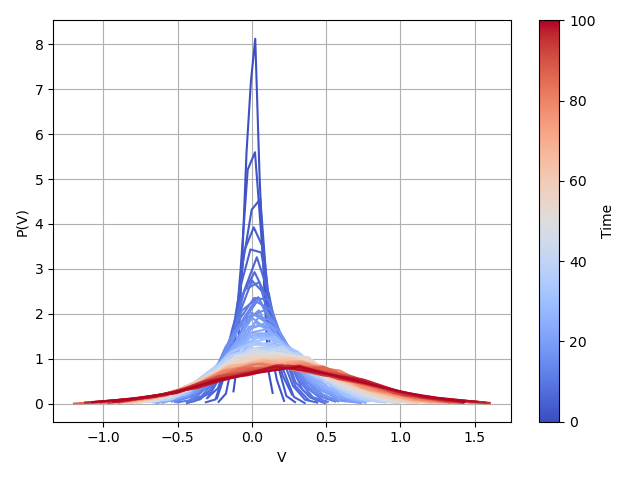
\includegraphics[width=80mm]{fig_1-A}}
\subfigure[]{\label{fig:b}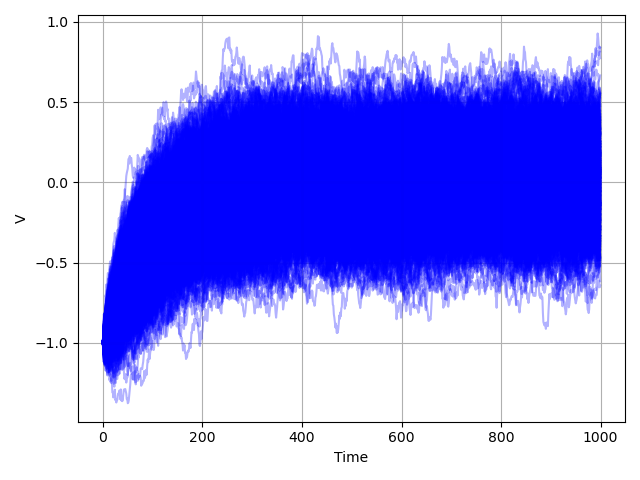
\includegraphics[width=80mm]{fig_1-B}}
\caption{Results of numerical integration of a Langevin equation for a gaussian white noise process with $\sigma = 1$, $\Delta t=0.002$, $\alpha=10$, and $V(0)=-1$. (a) Distribution of $V$ for $N=10,000$ units as a function of time (dashed is the theoretical prediction, solid is the simulation result). See stationary distribution in cyan (b) Time course for $N=10,000$ units}
\end{figure}


\section{Fokker-Planck for Homogeneous Sparse Networks}

The moments $M_{n}(t)$ derived above in the Kramers-Moyal expansion are dependent on the connectivity of the network and the statistics of the input. We will first consider a classic case, where we have a sparse directed network with constant synaptic efficacy between all presynaptic and postsynaptic pairs of cells. This primary pool of neurons is subject to stimulation by $N_{\mathrm{in}}$ input neurons with a connection probability $\gamma_{\mathrm{in}}$ giving $C_{\mathrm{in}} = \gamma_{\mathrm{in}}N_{\mathrm{rec}}$ unique connections between the input population and a single neuron in the recurrent pool. Within the recurrent pool, we have a connection probability of $\gamma_{\mathrm{rec}} << 1$ for any pair giving $C_{\mathrm{rec}} = \gamma_{\mathrm{rec}} N_{\mathrm{rec}}$ recurrent inputs per postsynaptic cell. We assume that a presynaptic action potential invokes a post synaptic potential (PSP) with magnitude $J_{0}$ in the postsynaptic cell with $J_{0} << \theta$ for both input and recurrent projections. The first moment of the transition operator $T(V',t| V,t-\tau)$ is given by

\begin{align*}
\mu(t) &= \mu_{in} + \mu_{rec}(t)\\
&= \left(C_{\mathrm{in}}\nu_{\mathrm{in}}(t) + C_{\mathrm{rec}}\nu_{\mathrm{rec}}(t)\right)\tau\langle J\rangle\\
&= \left(C_{\mathrm{in}}\nu_{\mathrm{in}}(t) + C_{\mathrm{rec}}\nu_{\mathrm{rec}}(t)\right)\tau J_{0}
\end{align*}

where $\nu_{\mathrm{in}}(t)$ is the rate parameter for the input Poisson process. The second moment

\begin{align*}
\sigma^{2}(t) &= \sigma_{\mathrm{rec}}^{2} + \sigma_{\mathrm{ext}}^{2}\\
&= \left(C_{\mathrm{in}}\nu_{\mathrm{in}}(t) + C_{\mathrm{rec}}\nu_{\mathrm{rec}}(t)\right)\tau\langle J^{2}\rangle\\
&= \left(C_{\mathrm{in}}\nu_{\mathrm{in}}(t) + C_{\mathrm{rec}}\nu_{\mathrm{rec}}(t)\right)\tau J_{0}^{2}
\end{align*}

After inserting the first two moments into (2.10) we arrive at the following Fokker-Planck equation

\begin{align*}
\dot{P}(V,t) &= -\frac{\partial}{\partial V}[\mu(t)P(V,t)] + \frac{1}{2}\frac{\partial^{2}}{\partial V^{2}}[\sigma^{2}(t)P(V,t)]\\
\end{align*} 

At this point, it is necessary to impose the appropriate boundary conditions on the above Fokker-Planck equation as in so as to maintain biological realism. The Fokker-Planck equation can be written as the continuity equation 

\begin{equation*}
\frac{\partial P(v,t)}{\partial t} = -\frac{\partial S}{\partial V}
\end{equation*}

(Risken, 1984) with 

\begin{equation*}
S(V,t) = -\frac{v-V_{L}-\mu}{\tau}P(V,t) - \frac{\sigma^{2}(t)}{2\tau}\frac{\partial P(V,t)}{\partial V}
\end{equation*}

which is known as the \emph{probability current} through voltage $V$ at a time $t$. The instantaneous firing rate is equivalent to the probability current through the threshold i.e. $\nu(t) = S(\theta,t)$. Furthermore, we require that the probability current through the firing threshold $P(\theta, t)=0$ and that instead this probability emerges at the resting potential after a refactory period of $\tau_{\mathrm{ref}}$. This condition gives the following boundary condition for the derivative of the probability with respect to voltage

\begin{equation*}
\frac{\partial P(\theta,t)}{\partial V} = -\frac{2\tau\nu(t)}{\sigma^{2}(t)}
\end{equation*}

To account for the refractory period $\tau_{\mathrm{ref}}$, we define an auxililary distribution

\begin{equation*}
p_{r}(t) = \int_{t-\tau_{\mathrm{ref}}}^{t} \nu(t)dt
\end{equation*}

which together with the distribution $P(V,t)$ satisfy the normalization condition:

\begin{equation*}
\int P(v,t)dV + p_{r}(t) = 1
\end{equation*}

\begin{align*}
\frac{\partial P(v,t)}{\partial t} &= \left(\mu(t) - \frac{v-v_{L}}{\tau}\right) \frac{\partial}{\partial v} P(v,t) - \frac{\sigma^{2}(t)}{2\tau}\frac{\partial^{2}}{\partial v^{2}} P(v,t) + \nu(t-\tau_{\mathrm{ref}})\delta(v-V_{R})\\
\end{align*} 


which we approximate by central finite differences

\begin{align*}
\frac{p(v, t+\Delta t) - p(v,t)}{\Delta t} &= \left(\mu(t) - \frac{v-v_{L}}{\tau}+ \mu_{ext}\right)\frac{p(v+\Delta v, t) - p(v,t)}{\Delta v} \\
&- \frac{1}{2}\left(\sigma^{2}(t) + \sigma_{ext}^{2}\right)\frac{p(v+\Delta v, t) - 2p(v,t) + p(v-\Delta v, t)}{\Delta v^{2}}
\end{align*} 


\chapter{Dynamical states of recurrent networks}
\section{Introduction}


\chapter{Stochastic computation by recurrent networks}
\section{Introduction}

\chapter{Conclusions}

% Intro to chapter one

% Format a LaTeX bibliography
\makebibliography

[1] Mculloch and Pitts. \textit{A logical calculus of the ideas imminent in nervous activity}. Journal of Mathematical Biophysics. 1943.

[2] J.J. Hopfield. \textit{Neural networks and physical systems with emergent collective computational abilities}. 1982.

[3] D.J. Amit. \textit{Spin-glass models of neural networks}. Physical Rev A. 1985.

[4] E. Gardner. \textit{The space of interactions in neural network models}. Journal of Physics A: Mathematical and General. 1988.

[5] N. Brunel. \textit{Dynamics of sparsely connected networks of excitatory and inhibitory neurons}. Journal of Computational Neuroscience. 2000. 

[6] Rosenbaum and Doiron. \textit{Balanced Networks of Spiking Neurons with Spatially Dependent Recurrent Connections}. Physical Review X. 2014.

[7] Zenke et al. \textit{Diverse synaptic plasticity mechanisms
orchestrated to form and retrieve memories
in spiking neural networks}. Nature Communications. 2015.

[8] Williams et al. \textit{Nonnegative decomposition of multivariate information}. arXiv. 2010.

[9] Amit et al. \textit{Storing infinite numbers of patterns in a spin-glass model of neural networks}. Physical Rev. Letters. 1985

[10] Nishimori. \textit{Statistical physics of spin glasses and information processing: an introduction}. Clarendon Press. 2010

[11] Buesing et al. \textit{Neural Dynamics as Sampling: A Model for Stochastic Computation in Recurrent Networks of Spiking Neurons}. PLOS Computational Biology. 2011

[12] Pecevski et al. \textit{Learning Probabilisitc Inference through Spike-Timing-Dependent Plasticitys}. eNeuro. 2016

[13] Pecevski et al. \textit{Formation and maintenance of neuronal assemblies through synaptic plasticity}. Nature Communications. 2014

[14] Pecevski et al. \textit{A learning algorithm for Boltzmann Machines}. Cognitive Science. 1985

% Figures and tables, if you decide to leave them to the end
%\input{figure}
%\input{table}

\end{document}


